\documentclass[12pt]{article}

\usepackage{amsmath}
\usepackage{graphicx}
\usepackage{geometry}
\usepackage{float}
\usepackage{setspace}
\usepackage{lmodern}
\usepackage{array}
\usepackage{caption}
\usepackage{ulem}
\usepackage{xcolor}

\geometry{margin=1in}
\setstretch{1.55}
\setlength{\parskip}{0.45em}

\setlength{\arrayrulewidth}{0.8pt}
\setlength{\tabcolsep}{12pt}
\renewcommand{\arraystretch}{1.5}

\begin{document}

\begin{center}
{\Huge\bfseries Parallel and Distributed Computing}\\[2cm]
{\LARGE\bfseries Assignment 7 - CUDA Programming and Profiling}
\end{center}

\vspace{2cm}

\noindent
{\Huge\underline{\textbf{PROBLEM 1}}}

\vspace{0.5cm}

{\Large\textbf{Different thread tasks for sum of first n integers}}

\vspace{1cm}

\textbf{Ques :}

Write CUDA program where threads do different task for summation of first n numbers for n = 1024. One task using iterative approach and one task using direct formula. Follow steps for host and device memory and kernel launch.

\vspace{0.7cm}

\textbf{\Large \underline{Output}}

\vspace{0.5cm}

Below is the terminal output for problem 1 run

\begin{figure}[H]
\centering
\fbox{
\includegraphics[width=0.95\textwidth]{outputs/output1.png}}
\caption*{\textbf{Figure 1: Problem 1 terminal output}}
\end{figure}

\vspace{0.8cm}

\textbf{\Large \underline{Observations}}

\vspace{0.5cm}

Graph is showing iterative and formula timing gap very clearly

\begin{figure}[H]
\centering
\fbox{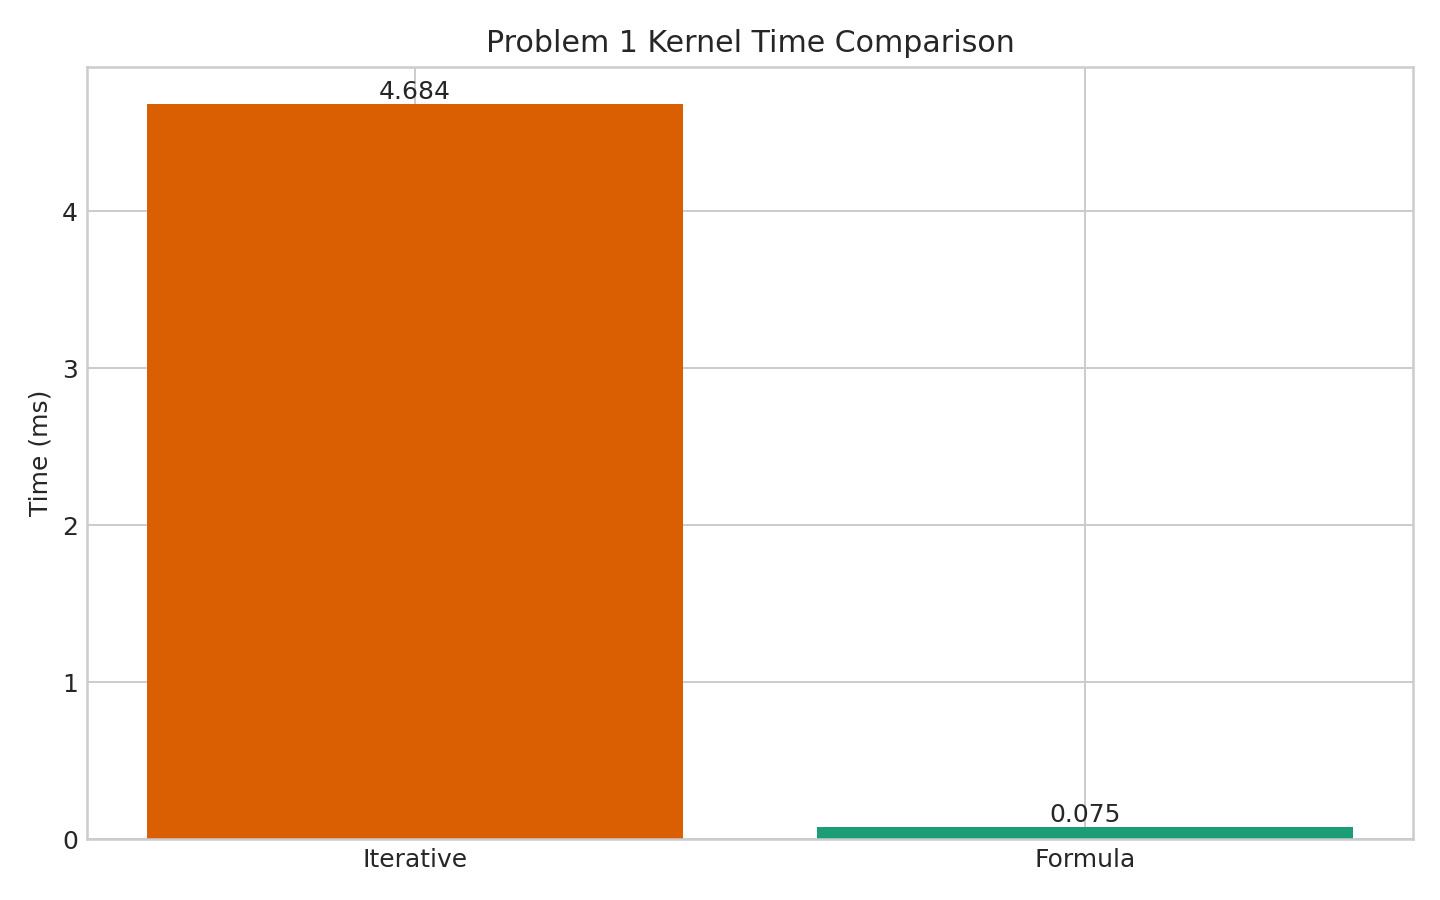
\includegraphics[width=0.85\textwidth]{outputs/problem1_time_compare.png}}
\caption*{\textbf{Figure 2: Problem 1 kernel time comparison}}
\end{figure}

Final sum for n = 1024 came same in both methods and table is below

\begin{center}
\begin{tabular}{|p{7cm}|p{5cm}|}
\hline
\textbf{Metric} & \textbf{Value} \\
\hline
Iterative sum output & 524800 \\
\hline
Formula sum output & 524800 \\
\hline
Iterative kernel time & 4.684224 ms \\
\hline
Formula kernel time & 0.074752 ms \\
\hline
Status & PASS \\
\hline
\end{tabular}
\end{center}

Both outputs matched for all threads so correctness is good

I also noticed that when thread value increases iterative method keeps doing more loop work so time keeps increasing internally

In formula method every thread does very small fixed amount of work so it stays fast and stable

Output table and graph together make it easy to see correctness and performance both in one glance

This kind of comparison is very useful because sometimes fast code gives wrong output but here both are correct

\vspace{0.8cm}

\textbf{\Large \underline{Inference}}

\vspace{0.5cm}

If same math can be done by direct formula then gpu threads save lot of time because loop work gets removed

So main learning is we should reduce per thread operations whenever possible because gpu runs huge number of threads

Iterative way is still important for understanding logic and for cases where no direct formula exists

But when formula exists it should be preferred for better performance and lower power usage also

This tells me algorithm choice matters as much as using gpu hardware

\vspace{0.8cm}

\textbf{\Large \underline{Conclusion}}

\vspace{0.5cm}

Problem 1 completed successfully both methods are correct but formula approach is clearly better for speed

All required steps were covered including host input device copy kernel launch and output verification

The result PASS for all threads confirms implementation is reliable for n equal to 1024

Final takeaway is direct formula based parallel kernel is the better solution for this specific task

\newpage

\noindent
{\Huge\underline{\textbf{PROBLEM 2}}}

\vspace{0.5cm}

{\Large\textbf{Merge sort for n = 1000 with pipelining and CUDA}}

\vspace{1cm}

\textbf{Ques :}

Implement merge sort for array of size n=1000

a. use pipelining for parallelization

b. implement parallel merge sort using CUDA

c. compare performance of both methods

\vspace{0.7cm}

\textbf{\Large \underline{Output}}

\vspace{0.5cm}

Below is terminal output for problem 2 run

\begin{figure}[H]
\centering
\fbox{
\includegraphics[width=0.95\textwidth]{outputs/output2.png}}
\caption*{\textbf{Figure 3: Problem 2 terminal output}}
\end{figure}

\vspace{0.8cm}

\textbf{\Large \underline{Observations}}

\vspace{0.5cm}

Graph is showing cpu pipelined vs cuda timing side by side

\begin{figure}[H]
\centering
\fbox{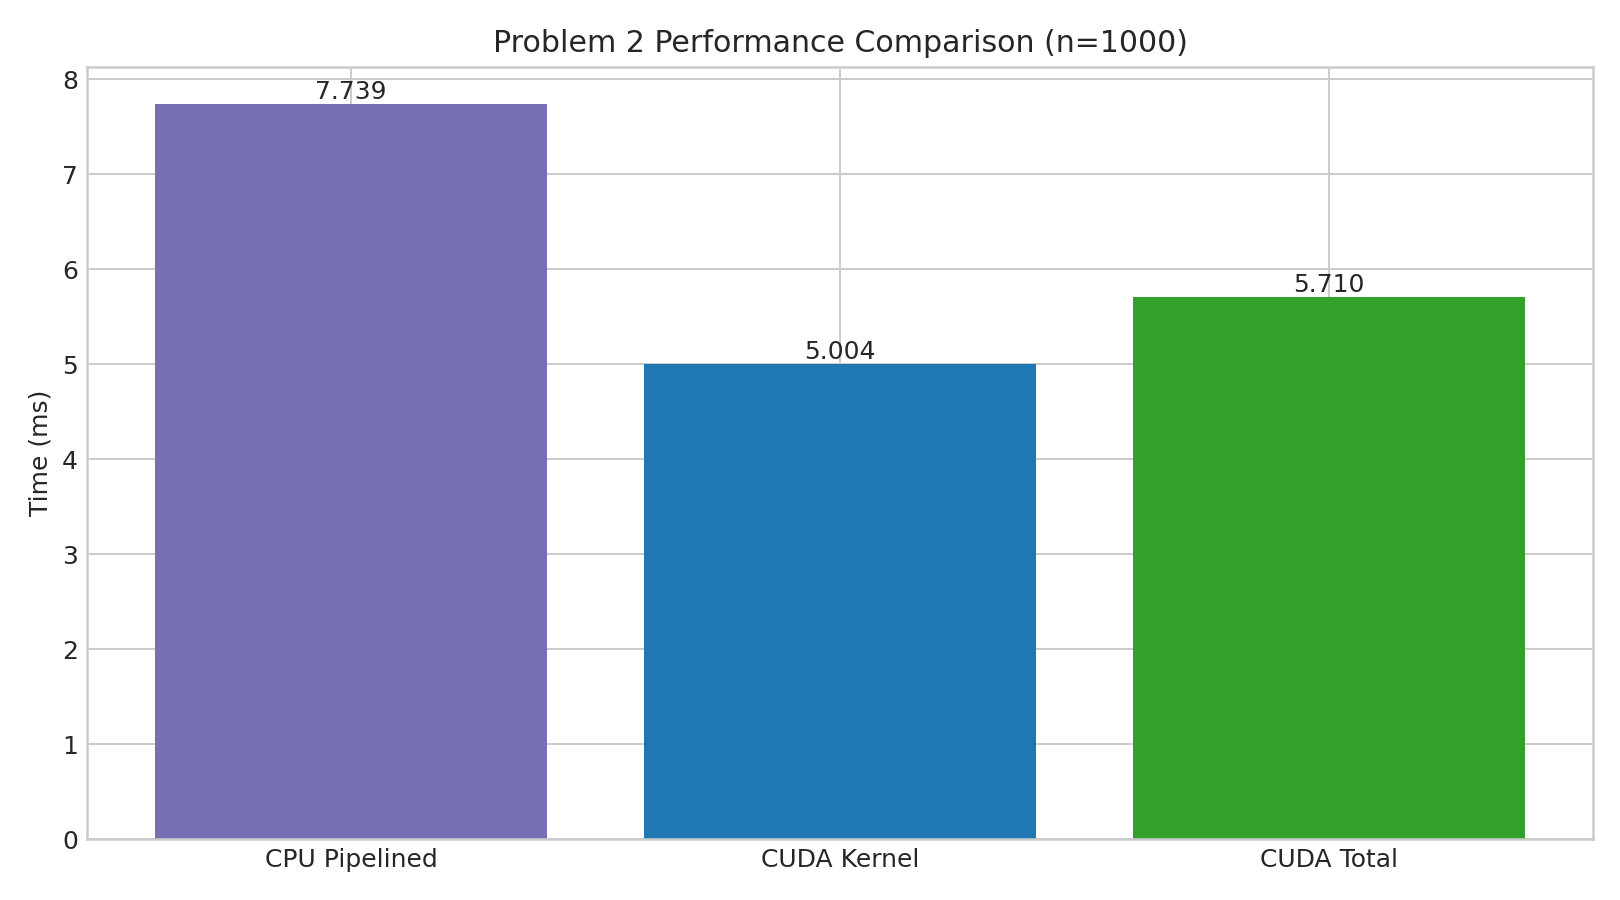
\includegraphics[width=0.88\textwidth]{outputs/problem2_time_compare.png}}
\caption*{\textbf{Figure 4: Problem 2 time comparison graph}}
\end{figure}

Table below shows full timing values and speedup

\begin{center}
\begin{tabular}{|p{7cm}|p{5cm}|}
\hline
\textbf{Metric} & \textbf{Value} \\
\hline
Input size & 1000 \\
\hline
CPU pipelined time & 7.739373 ms \\
\hline
CUDA kernel only time & 5.003584 ms \\
\hline
CUDA total time & 5.710112 ms \\
\hline
Speedup cpu/gpu total & 1.355380x \\
\hline
Status & PASS \\
\hline
\end{tabular}
\end{center}

Sorted values from both methods matched exactly so output is correct

In this run cuda total time is better than cpu pipelined time but margin is not very huge

I observed timing changes between runs also so single run should not be treated as absolute truth

For small n equal to 1000 transfer and launch overhead can still play a big role in total execution time

Graph and timing table are useful because they separate cpu time kernel time and total gpu time clearly

This made comparison fair and easy to explain in simple way

\vspace{0.8cm}

\textbf{\Large \underline{Inference}}

\vspace{0.5cm}

For n equals 1000 merge sort overhead still matters so huge gain should not be expected every time

Parallelization helps but only when workload is enough large to hide setup overhead

Pipeline style on cpu also gives improvement so gpu is not always the only fast option

Correctness check is very important because sorting output can look fine for first few values but still be wrong later

So inference is performance discussion must always include both speed and correctness

\vspace{0.8cm}

\textbf{\Large \underline{Conclusion}}

\vspace{0.5cm}

Problem 2 completed and both pipelined method and cuda method are working and giving same sorted output

Comparison part is also completed with proper measured values from actual run

For this input size result is moderate improvement not dramatic but still valid and meaningful

Overall implementation meets all asked parts a b and c in question 2

\newpage

\noindent
{\Huge\underline{\textbf{PROBLEM 3}}}

\vspace{0.5cm}

{\Large\textbf{Vector add with static symbols and bandwidth analysis}}

\vspace{1cm}

\textbf{Ques :}

Do basic vector addition and profile it. Then do changes:

1. use static global variables no cudaMalloc for device arrays

2. record kernel timing

3. query device props and compute theoretical bandwidth

4. compute measured bandwidth using bytes read write and kernel time

\vspace{0.7cm}

\textbf{\Large \underline{Output}}

\vspace{0.5cm}

Below is terminal output for vector add and timing details

\begin{figure}[H]
\centering
\fbox{
\includegraphics[width=0.95\textwidth]{outputs/output3.png}}
\caption*{\textbf{Figure 5: Problem 3 terminal output}}
\end{figure}

Profiler output is also added below

\begin{figure}[H]
\centering
\fbox{\includegraphics[width=0.95\textwidth]{outputs/output3_profiler.png}}
\caption*{\textbf{Figure 6: Profiler command output}}
\end{figure}

\vspace{0.8cm}

\textbf{\Large \underline{Observations}}

\vspace{0.5cm}

Bandwidth graph is showing ideal value and measured value gap

\begin{figure}[H]
\centering
\fbox{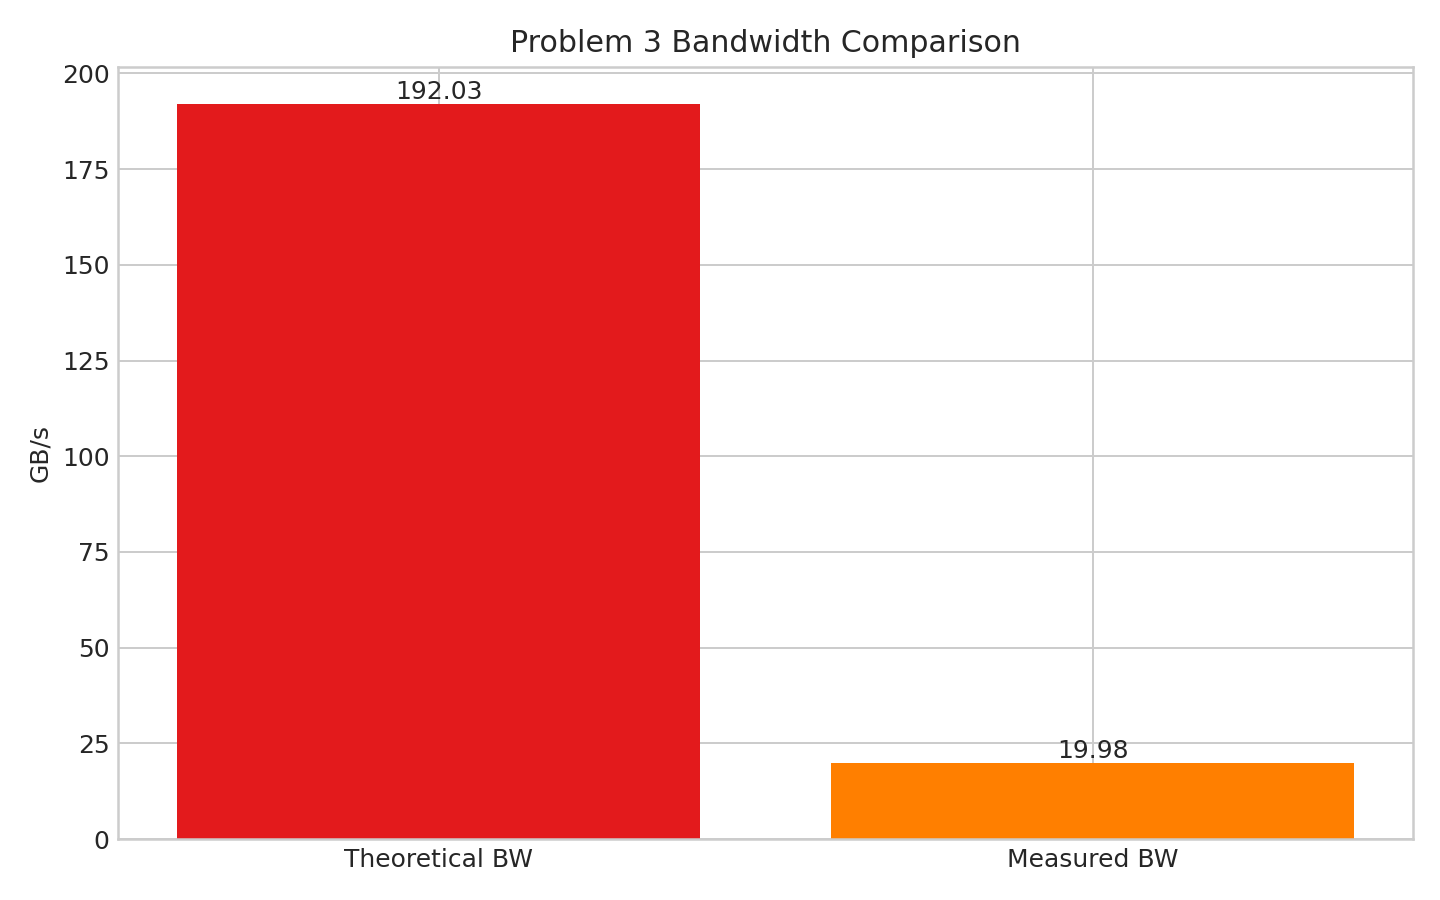
\includegraphics[width=0.82\textwidth]{outputs/problem3_bandwidth_compare.png}}
\caption*{\textbf{Figure 7: Problem 3 bandwidth graph}}
\end{figure}

For measured bandwidth this formula is used

$$
\text{Measured BW} = \frac{RBytes + WBytes}{t}
$$

Here each thread reads two float and writes one float so total bytes is

$$
(2 + 1) \times N \times 4
$$

Then divide by kernel time in seconds to get GB per second

Table below is showing measured and theoretical values

\begin{center}
\begin{tabular}{|p{7cm}|p{5cm}|}
\hline
\textbf{Metric} & \textbf{Value} \\
\hline
N value & 1,048,576 \\
\hline
Kernel time & 0.629920 ms \\
\hline
Theoretical bandwidth & 192.032 GB/s \\
\hline
Measured bandwidth & 19.975 GB/s \\
\hline
Measured/Theoretical ratio & 0.1040 \\
\hline
Status & PASS \\
\hline
\end{tabular}
\end{center}

Measured bandwidth is lower than theoretical and this is normal in real run

In this system nvprof and nsys were not in current path and output screenshot is showing this clearly

I also observed kernel time remains very small but measured bandwidth still far from theoretical peak value

This means hardware peak numbers are ideal and practical program gets limited by access pattern and runtime overhead

Table and graph both help to explain this gap in clear visual form so it becomes easy to discuss in viva

Static symbol approach worked correctly and PASS status confirms vector addition output is valid

\newpage

\textbf{\Large \underline{Inference}}

\vspace{1cm}

Static symbols plus event timing is enough to compute practical bandwidth nicely and compare with theoretical limit

From this experiment i can infer that timing and bandwidth numbers should always be reported together

Only kernel time without byte level analysis does not show full memory behavior of kernel

Even simple vector add can be memory bound and that is why measured bandwidth becomes key metric

So profiling mindset means checking both what is possible in theory and what is achieved in real execution

\vspace{1cm}

\textbf{\Large \underline{Conclusion}}

\vspace{1cm}

Assignment 7 is completed all three problems are running fine outputs are saved graphs are added tables are added and observations inference conclusion are written in simple way

Problem 1 showed direct formula based kernel is much faster while giving same correct result

Problem 2 showed parallel merge methods on cpu and gpu both are useful and comparison depends on input size

Problem 3 gave practical understanding of timing theoretical bandwidth and measured bandwidth gap

Overall this assignment improved both cuda coding confidence and performance analysis understanding in a very practical way

\vspace{2cm}

\textbf{Submitted to :} Dr Saif Nalband

\textbf{Submitted by :} Arpan Goyal

\textbf{Roll No. :} 102303479

\end{document}
